\chapter{实验评估}
\label{chap:evaluation}
本章中,我们通过在两个比较有代表性的数据集上进行实验来对我们的系统进行各方面的评估。我们的主要评估手段是比较我们的系统和直接计算之间的性能差异,以及比较这两种方式能够处理数据的规模。

首先,我们介绍了实验使用的数据集的概括以及所用的实验环境。然后,我们对树状结构证明进行了单独的实验评估。我们通过比较用树状结构证明的方式生成正确性证明和直接计算正确性证明的时间效率,来评估树状结构证明带来的性能提升。接着,我们对系统的整体性能做了实验评估,使用的是任务的总时间,包括搜索时间、生成正确性证明的时间、生成可靠性证明的时间作为评估指标。然后,我们对于结果证明的验证时间以及基于采样的验证机制进行了实验评估。最后,我们测试评估了系统中在处理大数据集情况下的表现。

\section{数据集}

在我们这次的实验评估中,我们使用了两个数据集:一个是Enron Email, 另一个是Wikipedia。

Enron Email:该数据集是一些用户电子邮件的合集,都是一些txt格式的文本文件。该数据集有着类似一般用户日常使用的规模。我们选择了其中用户Mann-k的电子邮件,用来测试我们的系统在一般用户日常使用时的性能表现。

Wikipedia:该数据集是维基百科的英文版本数据集,文档内容是以HTML格式的文本文件进行存储的。该数据集数据规模较大,在我们的测试环境里无法使用直接计算的方式进行处理。我们使用该数据集来测试我们的系统在处理大规模数据时的表现。

在表\ref{tab:dataset_stat}里,我们给出了这两个数据集的一些数据概况。在每个数据集上我们都选择了一些比较费时间的查询来进行考验效率的情况下的测试,同时我们也随机选择了一些常见的查询来进行一般情况下的性能测试。
\begin{table}[htb]
    \centering
    \bicaption[tab:dataset_stat]{表}{数据集的概况}{Tab.}{Statistics of datasets}
    \begin{tabular}{cccccc}
        \toprule
        数据集 & 文档数目 & 词条数目 & 大小 \\
        \midrule
        Enron & 46,762 & 69,937 & 100MB  \\
        Wikipedia & 14,257,486 & 13,320,882 & 101GB  \\
        \bottomrule
    \end{tabular}
\end{table}

\section {测试环境}

我们的测试环境是一个包含12台机器的集群。
我们的测试不包含系统的启动时间,在系统启动好后,不再进行文件的读写操作,所以硬盘速度的影响我们不考虑。我们使用了该集群搭建的NAS来存储我们的索引文件和事先计算的数据,而不使用本地磁盘。所以在这里我们就不关注本地的磁盘配置了。每台机器的配置如下:

\begin{itemize}
    \item \textbf{CPU} 2个Intel E5645 2.40GHz
    \item \textbf{内存} 64GB
    \item \textbf{网络} 1000Mbps
\end{itemize}

\section {正确性证明的性能比较}
\begin{table}[htb]
    \centering
    \bicaption[tab:correctness_speedup]{表}{正确性证明的生成速度提升}{Tab.}{The Speedup of Building Correctness Proof}
    \begin{tabular}{cccccc}
        \toprule
        查询编号 & 直接计算时间(s) & 树状证明时间(s) & 速度提升 \\
        \midrule
        1 & 1.177 & 0.672 & 1.752  \\
        2 & 8.931 & 1.272 & 7.022  \\
        3 & 0.703 & 0.387 & 1.818  \\
        4 & 1.267 & 0.823 & 1.540  \\
        5 & 1.631 & 0.987 & 1.653  \\
        6 & 1.016 & 0.649 & 1.565  \\
        \midrule
        平均 & 2.454 & 0.798 & 2.558  \\
        \bottomrule
    \end{tabular}
\end{table}

由于本实验的数据规模不是很大,我们是使用一台集群中的机器进行。实验的数据结果如表\ref{tab:correctness_speedup}所示。从实验结果来看,我们的树状结构证明方式相比于直接计算大概有着2.5倍左右的提升。对于那些计算时间比较长的查询,我们的方式的提升效果更加明显。比如说这次实验中的查询2,使用的关键词是message和queue,其中message对应的倒排索引数据的大小为46762,queue对应的倒排索引数据的大小为188。最后搜索结果集合的大小是188,说明这里恰巧包含queue的文档都包含message这个关键词。对于这么大的集合,用直接计算的方法,生成正确性索引需要8.931秒,而用我们的树状结构证明方式则只需要1.272秒。这可以说明,树状结构证明比较适合处理集合元素比较多的情况。

\section {总体性能测试}

\begin{table}[htb]
    \centering
    \bicaption[tab:overall_speedup]{表}{总体提升}{Tab.}{The overall speedup}
    \begin{tabular}{cccccc}
        \toprule
        查询编号 & 直接计算时间(s) & 本系统时间(s) & 速度提升 \\
        \midrule
        1 & 1.819 & 0.840 & 2.165 \\
        2 & 9.051 & 2.278 & 3.973 \\
        3 & 1.066 & 0.498 & 2.143 \\
        4 & 1.984 & 1.064 & 1.866 \\
        5 & 2.497 & 1.272 & 1.962 \\
        6 & 1.512 & 0.801 & 1.888 \\
        \midrule
        平均 & 2.988 & 1.125 & 2.333 \\
        \bottomrule
    \end{tabular}
\end{table}

我们使用了Enron Email数据集在一台机器上进行了本次测试。
测试结果如表\ref{tab:overall_speedup}中所示。从测试结果中,我们可以看出我们的系统相比于直接计算的方式有着差不多2倍的速度提升。由于我们采用了正确性证明和完整性证明并行计算的方法,我们的系统的计算时间主要取决于正确性证明和完整性证明中计算的比较慢的那个。而直接计算时,总的时间是这两个部分证明的计算时间之和。在大部分情况下,这两个部分的证明计算时间都差不多,所以我们的系统的提升倍数也在2倍左右。对于查询2,得益于树状证明在正确性证明计算上带来的巨大提升,总体性能有着比别的查询更加明显的提升。

\section{验证时间的比较}
\begin{table}[htb]
    \centering
	\bicaption[tab:verifying_time]{表}{结果证明的验证时间}{Tab.}{Verification time}
    \begin{tabular}{cccccc}
        \toprule
        查询编号 & 本系统(s) & 直接计算(s) \\
        \midrule
        1 & 0.520 & 0.452 \\
        2 & 0.271 & 0.197 \\
        3 & 0.492 & 0.442 \\
        4 & 3.532 & 3.241 \\
        5 & 4.705 & 4.324 \\
        6 & 0.979 & 0.904 \\
        \midrule
        平均 & 1.750 & 1.593 \\
        \bottomrule
    \end{tabular}
\end{table}
为了测试在提升了证明生成速度之后,我们的系统会不会对证明的验证速度有着不好的影响,我们使用Enron数据集进行了验证时间的测试。
测试结果如表\ref{tab:verifying_time}中所示。
从测试结果中,我们可以看出我们的系统的证明验证速度比直接计算有着大约10\%左右的降低,
这个程度的降低相比较证明速度的提升是完全可以接受的。
本系统验证速度降低的主要原因是使用了树状证明,使得正确性验证需要多验证一些Membership Witness。还有,这里的证明验证没有使用事先计算的质数,所以每次验证都要计算大量的质数表示,这导致了证明验证的时间和证明生成的时间都差不多了。我们可以让云端在返回搜索结果的同时返回签了名的相应的质数表示,这样用户在证明验证的时候就不需要再进行质数表示的计算了。当然,这样会增加返回结果的大小。对这里的权衡关系,本课题没有进行深入的研究。
\section{基于采样的验证机制的性能和正确性保证}
\begin{figure}[htb]
\centerline{
\begin{tikzpicture}
\begin{axis}[
    xlabel={$r$},
	ylabel={$t(s)$},
	yticklabel style={/pgf/number format/fixed,
	    /pgf/number format/precision=1},
	xticklabel={\pgfmathparse{\tick*100}\pgfmathprintnumber{\pgfmathresult}\%},
	xticklabel style={/pgf/number format/fixed,
	    /pgf/number format/precision=0},
	xmin = 0,
	xmax = 1.0,
	ymin = 0,
	%ymax = 1.0,
]
\addplot[blue,smooth,mark=*] coordinates 
{ 
(0, 0.0305)
(0.1, 0.149)
(0.2, 0.2515)
(0.3, 0.369)
(0.4, 0.4705)
(0.5, 0.594)
(0.6, 0.7075)
(0.7, 0.808)
(0.8, 0.9345)
(0.9, 1.049)
(1, 1.1555)
};
\addplot[black,densely dashed] coordinates
{
(0, 1.125)
(1, 1.125)
}[yshift=8pt]
node[pos=0.2]{验证搜索时间}
;
\addplot[black,densely dashed] coordinates
{
(0, 0.03)
(1, 0.03)
}[yshift=8pt]
node[pos=0.75]{非验证搜索时间}
;
\end{axis}
\end{tikzpicture}
}
\bicaption[fig:rateTime]{图索引}{不同采样率下的平均搜索时间}{Fig}{Average search time on different sampling rates}
\end{figure}

在前面章节我们提出了一种基于采样的验证机制,使得用户可以在性能和正确性保证之间做出权衡。在这里,我们对该机制进行了性能的实验评估和正确性保证的测试。

在基于采样的验证机制里面,验证搜索只是用来验证云服务商的正确性,非验证搜索才是用户真正需要的搜索请求,所以在这里我们把非验证搜索的数目称之为有效搜索数。
这里我们令采样率r为验证搜索次数(也就是采样数)x和非验证搜索次数(也就是有效搜索数)n的比例:$r = x/n$。

我们使用了Enron数据集对不同采样率下的平均搜索时间进行了测试。这里的平均搜索时间为总的时间除以有效搜索的次数。测试结果如图\ref{fig:rateTime}所示。从图中的结果来看,随着采样率的不断增加,平均的搜索时间在呈线性地不断增长。由于多了非验证搜索的时间代价,当采样率接近100\%时,基于采样的验证机制的平均搜索时间将超过验证搜索时间。在采样率比较低的时候,基于采样的验证机制相比验证搜索是有着明显的时间效率提升。比如当采样率为10\%时,基于采样的验证机制的平均搜索时间为0.143秒,相比于验证搜索的平均时间1.13秒有着8倍左右的速度提升。
\begin{figure}[htb]
\centerline{
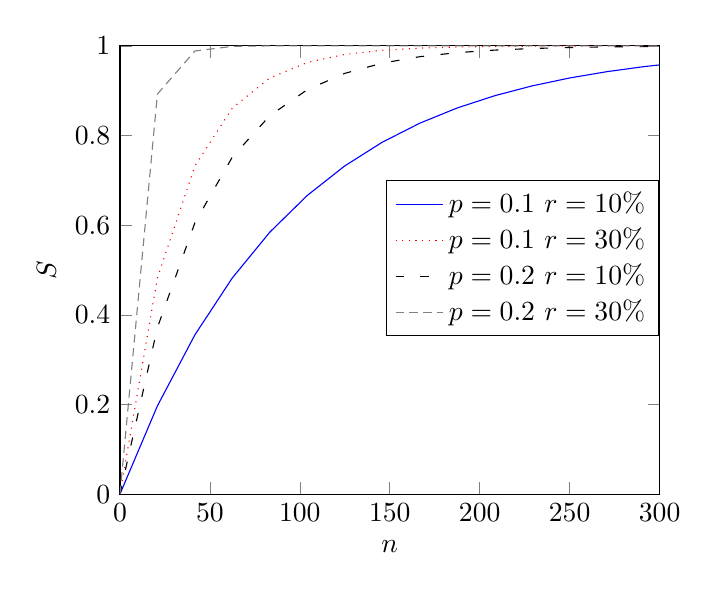
\begin{tikzpicture}
\begin{axis}[
    xlabel={$n$},
	ylabel={$S$},
	yticklabel style={/pgf/number format/fixed,
	    /pgf/number format/precision=1},
	xticklabel style={/pgf/number format/fixed,
	    /pgf/number format/precision=0},
	xmin = 0,
	xmax = 300,
	ymin = 0,
	ymax = 1.0,
	legend entries= {
	  $p=0.1\ r=10\%$, 
	  $p=0.1\ r=30\%$, 
	  $p=0.2\ r=10\%$,
	  $p=0.2\ r=30\%$,
	},
	legend style={at={(1,0.7)},anchor=north east}
]
\addplot[blue,solid,domain=0:500] { 1-exp(x*0.1*ln(1-0.1)) };
\addplot[red,dotted,domain=0:500] {1-exp(x*0.3*ln(1-0.1))};
\addplot[black,loosely dashed,domain=0:500] {1- exp(x*0.1*ln(1-0.2)) };
\addplot[gray,densely dashed,domain=0:500] { 1-exp(x*0.3*ln(1-0.3)) };
\end{axis}
\end{tikzpicture}
}
\bicaption[fig:ratePoss]{图索引}{一些情况下的正确性保证和有效搜索次数的关系}{Fig}{The relation between the assurance and query times}
\end{figure}

我们在图\ref{fig:ratePoss}中绘制了在几种特定云服务商欺骗率p和采样率r的情况下,用户能成功发现云服务商有问题的概率S和用户进行的有效搜素次数n的关系。这里,$S = 1 - (1-p)^{n \times p}$。从图中我们可以看出,随着搜索次数的增多,用户能发现云服务有问题的概率呈指数级增长。在云服务商欺骗率固定的情况下,采样率越高,正确性保证越高。在系统的实际使用中,我们可以考虑动态的调整采样率,比如说刚开始的时候使用较高的采样率,以期望能在更早的时候发现云服务是不是有问题,之后的使用中,可以降低采样率来取得更好的性能。同时,我们可以考虑将一些采样验证放在系统空闲时间进行,比如说放在深夜。

\section {大数据集的性能测试}
\begin{table}[htb]
    \centering
	\bicaption[tab:wiki_speedup]{表}{Wikipedia数据集上的性能测试结果}{Tab.}{The performance on dataset wikipedia}
    \begin{tabular}{cccccc}
        \toprule
        查询编号 & 耗时(s) \\
        \midrule
        1 & 706.038  \\
        2 & 8.096  \\
        3 & 209.649  \\
        4 & 7.677  \\
        5 & 770.438  \\
        6 & 87.117  \\
        \midrule
        平均 & 298.169  \\
        \bottomrule
    \end{tabular}
\end{table}
本测试我们使用的是Wikipedia数据集,在10台机器上进行。
各台机器上的模块部署情况如下:
\begin{itemize}
\item 机器0:Search Client、Search Server
\item 机器1:Correctness Server
\item 机器2:Integrity Server
\item 机器3 - 9:Query Node
\end{itemize}

测试结果如表格\ref{tab:wiki_speedup} 所示。从测试结果中,
我们可以看出我们的系统能够对100GB数据规模的数据集进行处理,
但处理速度还不是很好,而且不同查询的处理速度有着很大的变化。
对于有些查询,我们的系统能够在10秒内给出结果,而对于一些别的查询,
处理时间却长达10分钟。这主要的原因是,这些查询关键词的文档集合都是在百万千万级别的,且不同的关键词之间的文档集合差异很大。
对于这么大的集合,我们系统计算结果证明的速度还有待提高。

\section{本章小结}
在本章我们对云搜索正确性快速验证系统进行了一系列的实验评估。我们的实验使用了两个比较有代表性的数据集:Enron Email和Wikipedia。对系统的实验评估主要通过比较我们的系统和直接计算之间的性能差异进行。

首先,我们比较了使用树状结构证明前后正确性证明生成时间上的差异,实验结果表明使用树状结构证明对正确性证明生成速度有大约2.5倍的提升。接着,我们测试了系统的整体性能表现。实验结果表明我们的系统比直接计算的方法有着差不多2倍的性能提升。然后,我们比较了使用树状结构证明前后的验证时间差异。实验结果表明,使用了树状结构证明之后,验证时间有10\%左右的增加,处在可以接受的程度范围内。接着,我们对基于采样的验证机制进行了性能测试。实验结果表明使用了采样验证之后,系统的性能有着较大的提高。比如在10\%采样率时,系统的性能有着8倍左右的提高,而此时的系统正确性保证也是不错的。最后,我们在大数据集上进行了性能测试,测试结果表明我们的系统能够在大数据集上正常使用,但系统的效率还不够高。
